\Exhibit{GitCommit}{%
    Screenshot of a GitHub help page explaining what a commit is%
}

This screenshot shows the top of the GitHub help page that explains
what a commit is,

\ParagraphQuote{%
    which is like a snapshot of your repository.
    These commits are snapshots of your entire repository at specific times.
    You should make new commits often, based around logical units of change.
    Over time, commits should tell a story of the history of your repository
    and how it came to be the way that it currently is.%
}

This proves that the number of commits is a metric of developers' activity on a project,
which correlates with the importance of a project.

\begin{center}
    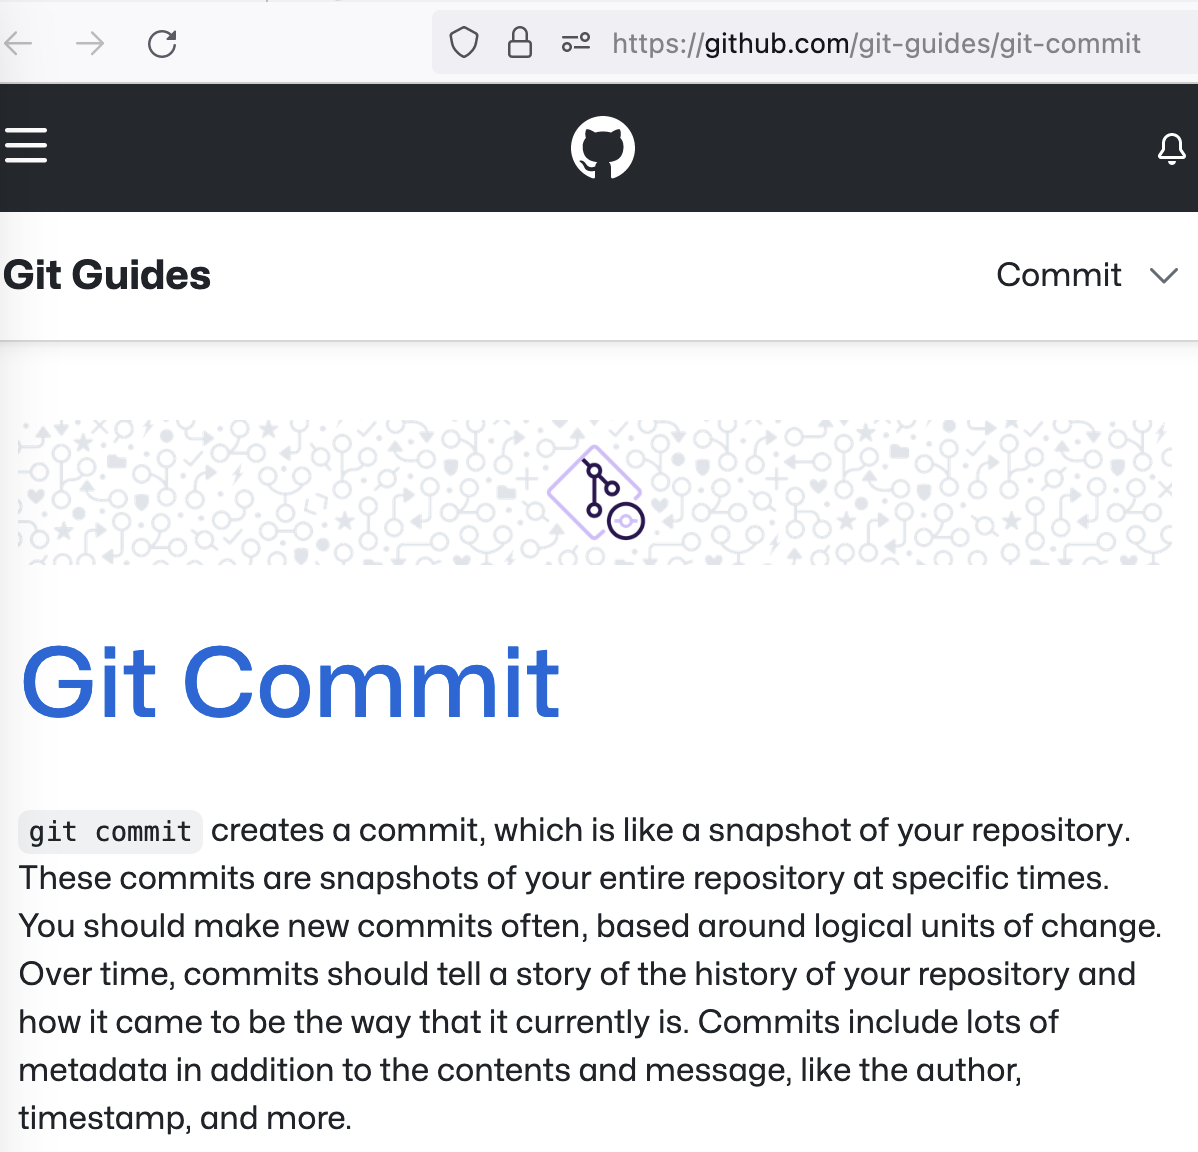
\includegraphics[width=35em]{git-commit}
\end{center}

\pagebreak
